\documentclass{beamer}
\usepackage{ctex}
\usepackage{zhs}
\usepackage{diagbox}  % 斜线表头
\usepackage{colortbl} %
\title{python语言程序设计基础}
\author{Hengsheng Zhou}
\institute{电信与智能制造学院}
\begin{document}
\begin{frame}[t]
	\titlepage
	\begin{figure}
		\begin{center}
			\includegraphics[width=0.2\linewidth]{output.eps}
		\end{center}
	\end{figure}


\end{frame}
\begin{frame}
	\frametitle{Outline}
	\tableofcontents
\end{frame}
\section{说课内容}

\subsection{为什么学python}

\begin{frame}[t]
	1. Python 用途广泛,生态丰富,无论是初学者还是专业开发者,都能在不同领域找到合适的应用场景!
	\pause
	\begin{table}[h]
		\centering
		\begin{tabular}{|c|c|c|c|}
			\hline
			\diagbox{应用场景}{示例} & 框架                        \\
			\hline
			数据分析               & Matplotlib/Seaborn(数据可视化) \\
			\hline
			自动化                & 批量文件处理                    \\
			\hline
			数据采集               & Scrapy                    \\
			\hline
		\end{tabular}
	\end{table}
	\pause
	2. Python 语法简洁、易学易用,适合零基础入门.
	\pause
	\begin{center}
		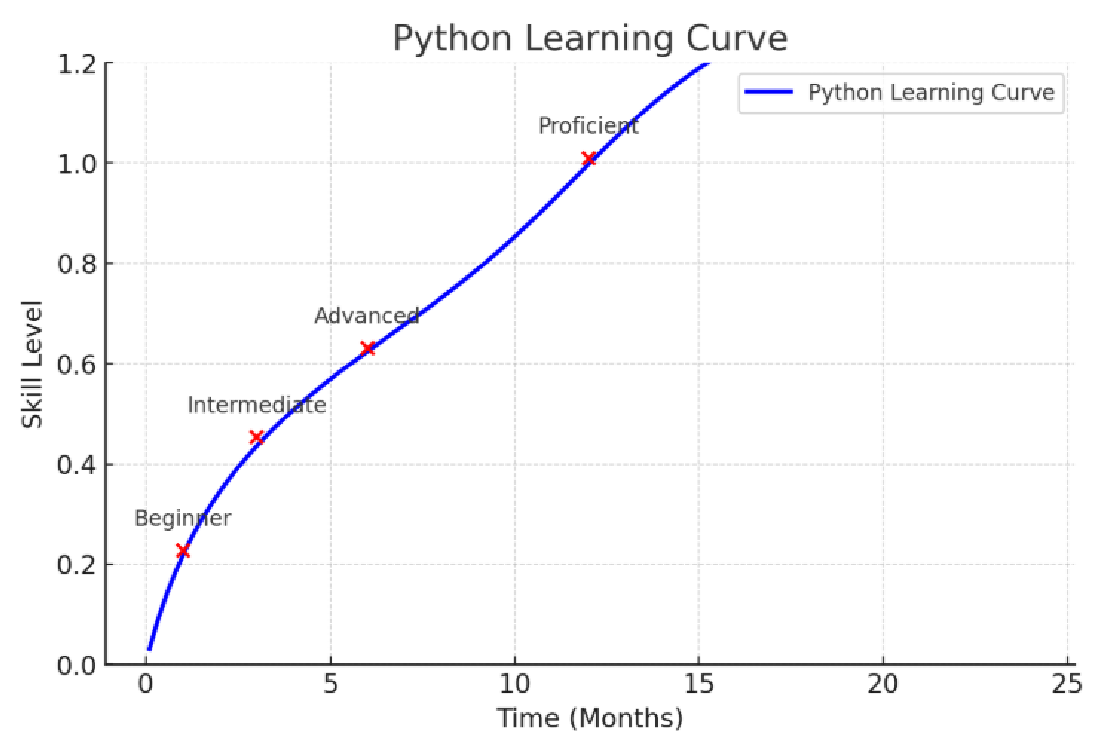
\includegraphics[width=0.5\linewidth]{learning_curve.eps}
	\end{center}

\end{frame}
\subsection{学情分析}


\begin{frame}[t]
	\begin{columns}
		\begin{column}{0.7\textwidth}
			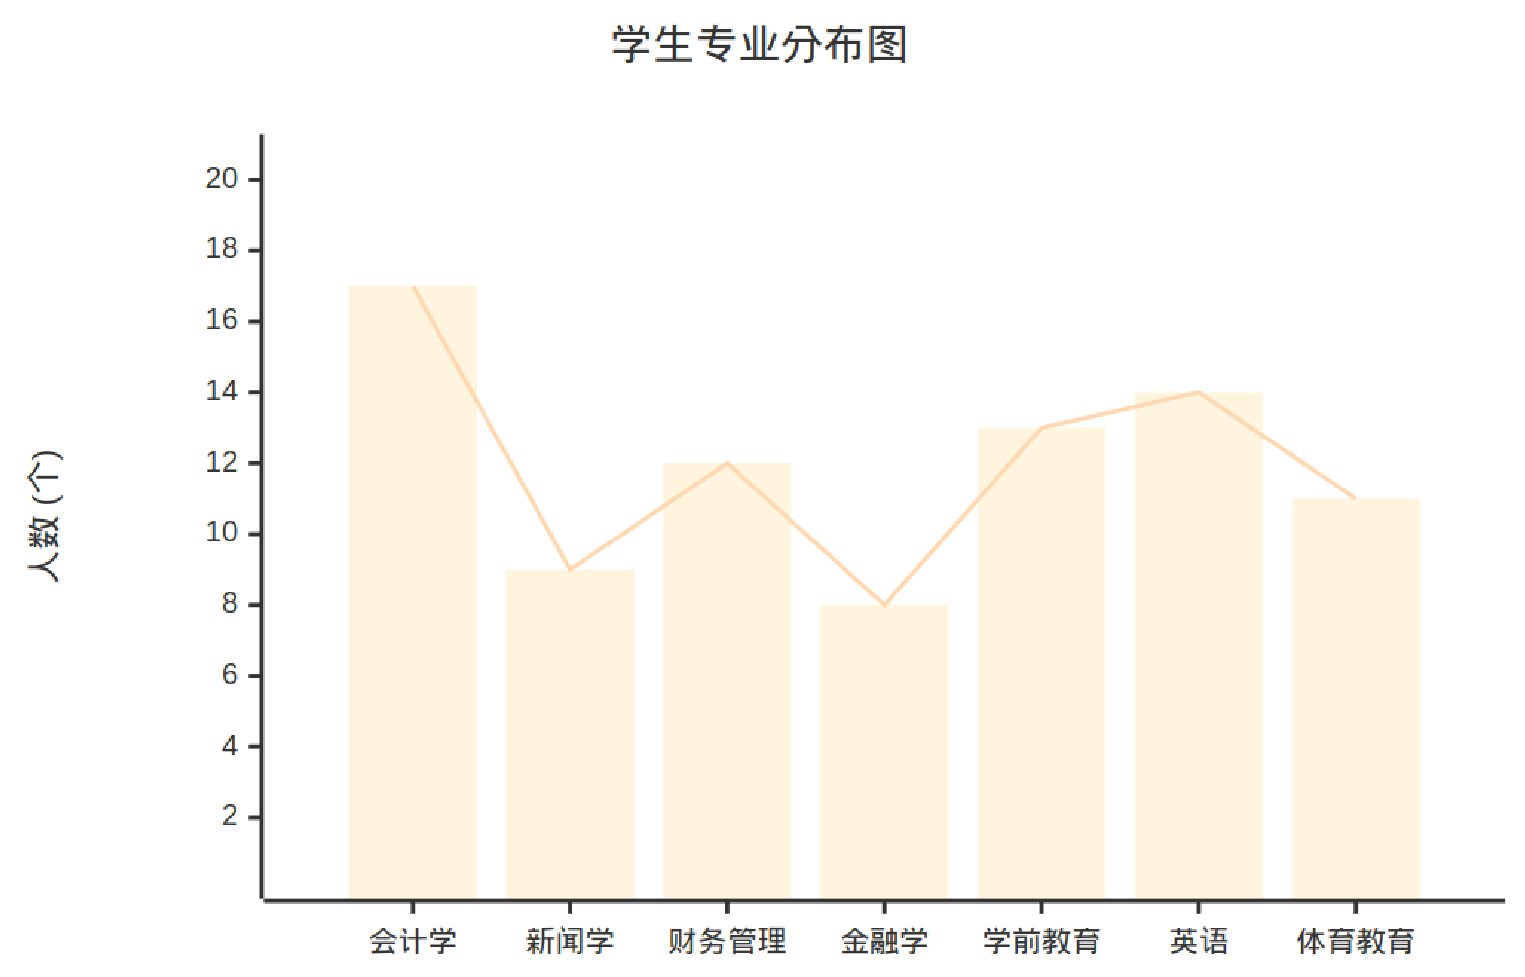
\includegraphics[width=0.8\linewidth]{student_number.eps}
		\end{column}
		\pause
		\begin{column}{0.3\textwidth}
			\begin{itemize}
				\item 学生分布于多个专业
				\item 大多数学生为非计算机专业,不具有相关背景知识
			\end{itemize}
		\end{column}
	\end{columns}
	\pause
	\begin{columns}
		\begin{column}{0.7\textwidth}
			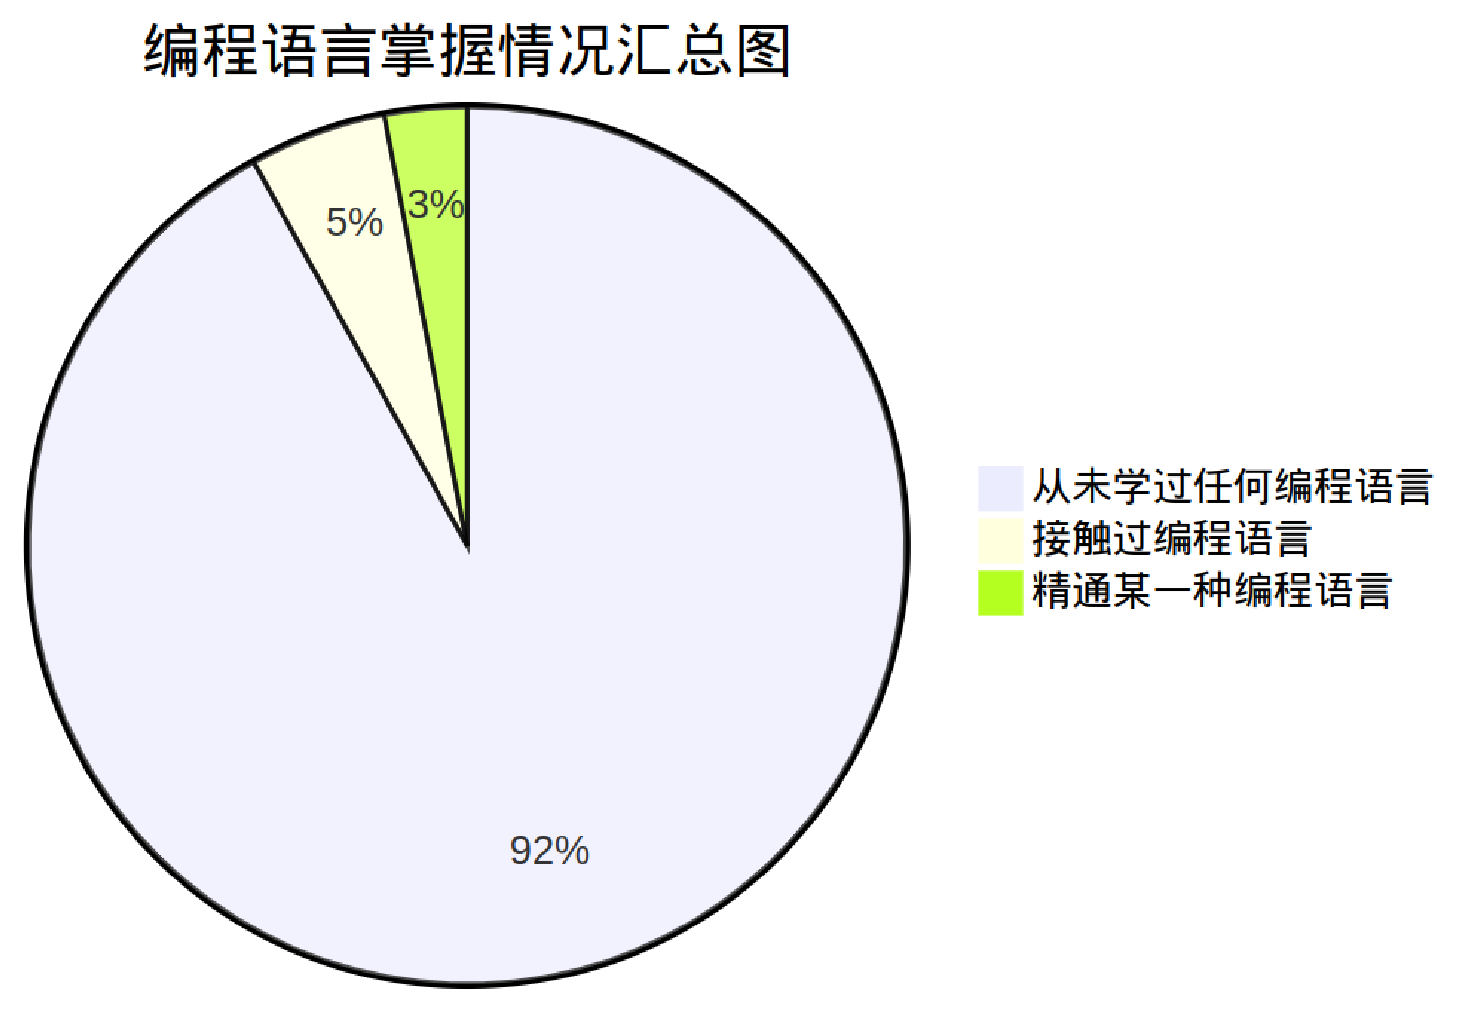
\includegraphics[width=0.7\linewidth]{pie.eps}
		\end{column}
		\pause
		\begin{column}{0.3\textwidth}
			\begin{itemize}
				\item 大多数学生在学习之前没有接触过任何编程语言,属于零基础

			\end{itemize}
		\end{column}
	\end{columns}

\end{frame}

\subsection{如何开展教学工作}

\begin{frame}[t]
	\begin{itemize}
		\item<1-> 避免陷入“理论陷阱”
		      \pause
		      \begin{alertblock}{solution}
			      学一点就写代码,实践出真知,避免只看不练
		      \end{alertblock}
		      \pause
		\item<2-> 先掌握最基础的知识
		      \pause
		      \begin{alertblock}{solution}
			      遇到复杂的问题就先跳过,由浅入深
		      \end{alertblock}
		      \pause
		\item<3-> 熟练使用AI辅助工具
		      \pause
		      \begin{alertblock}{solution}
			      学会使用deepseek,ChatGPT等AI辅助工具编写代码
		      \end{alertblock}
		      \pause
		\item<4-> 找python开发社区交流经验
		      \pause
		      \begin{alertblock}{solution}
			      学习在GitHub和Stack Overflow等开源社区寻找学习资源
		      \end{alertblock}



	\end{itemize}

\end{frame}
\subsection{AI与信息化技术赋能课堂}
\begin{frame}[t]
	\begin{columns}
		\begin{column}{0.5\textwidth}
			1. 使用信息化工具padlet向学生发布课堂讨论问题
			\pause
			\begin{example}
				如何用python在数据库中创建一个数据表?

			\end{example}
			\pause
		\end{column}
		\begin{column}{0.5\textwidth}
			\begin{figure}[htpb]
				\centering
				
\includegraphics[width=0.5\textwidth]{QRcode.eps}
				\label{fig:}
			\end{figure}
		\end{column}
	\end{columns}
	\pause
	\begin{figure}[htpb]
		\centering
		\includegraphics[width=0.9\textwidth]{discussion.png}
		\label{fig:discussion}
	\end{figure}

\end{frame}

\begin{frame}[t]

	2. 根据收集到的学生讨论信息使用AI生成代码。
	\pause
	\begin{figure}[htpb]
		\centering
		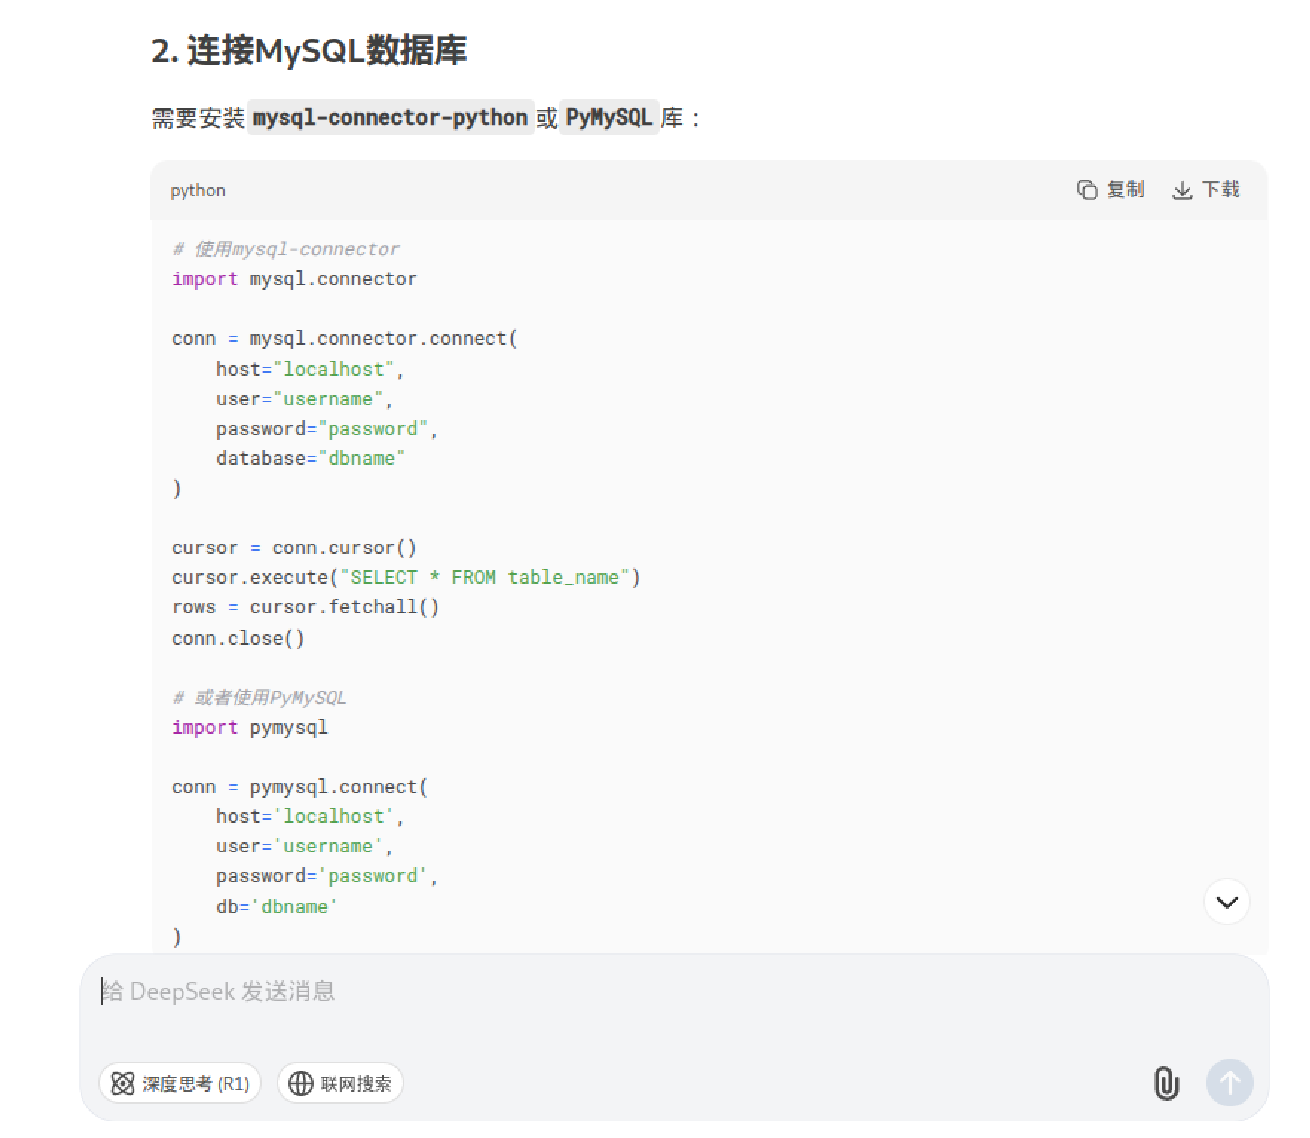
\includegraphics[width=0.5\textwidth]{deepseek.eps}
		\label{fig:deepseek-eps}
	\end{figure}
	\pause
	\begin{alertblock}{调试}
		通常AI生成的代码无法直接运行,需要视具体情况带领学生一步步的调试代码

	\end{alertblock}

\end{frame}
\subsection{课程思政}

\begin{frame}[t]
	在专业课程教学中融入思政教育,实现知识传授和价值引导的统一,是教学过程中不可或缺的重要环节,课程思政教育贯穿本课程教学全过程。
	\begin{figure}[htbp]
		\begin{center}
			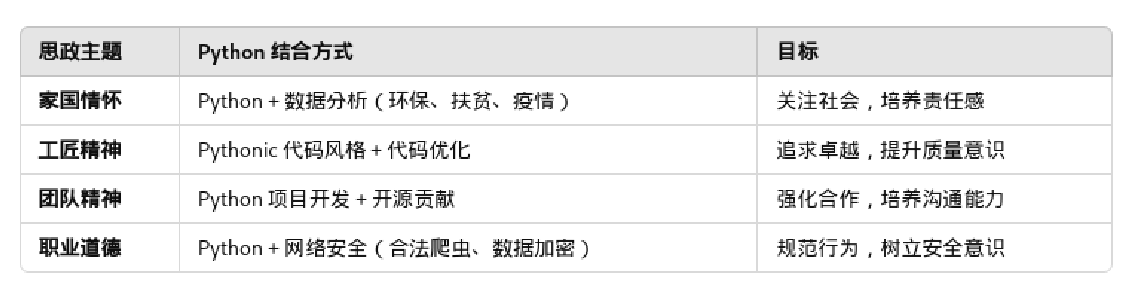
\includegraphics[width=0.9\linewidth]{policy.eps}
		\end{center}
	\end{figure}
	\pause
	不同思政目标所对应的实现方式
	\begin{center}
		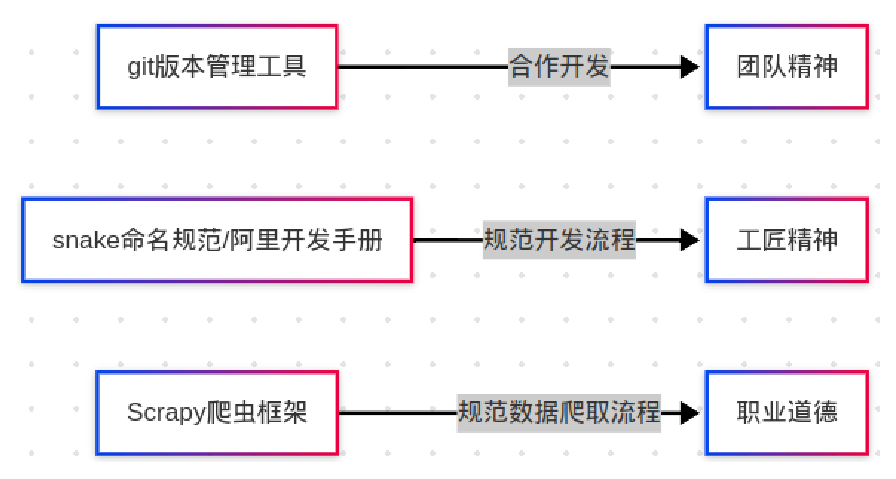
\includegraphics[width=0.5\linewidth]{tools_for_policy.eps}
	\end{center}
\end{frame}


\end{document}
